\chapter{Instrukcja użytkownika}

Poniższy rozdział opisuje wymagania oraz kroki konieczne do zbudowania oraz uruchomienia projektu.
Zdefiniowane wymagania wstępne opisują przetestowaną konfigurację, dla której aplikacja działa w 100\% poprawnie.
Możliwe, że będzie ona działać poprawnie także przy innej konfiguracji, szczególnie dla nowszych wersji bibliotek i środowisk uruchomieniowych, ale nie ma takiej pewności.

\section{Wymagania wstępne}

\begin{itemize}
	\item W systemie operacyjnym konieczne jest zainstalowanie środowiska Java Runtime Environment w wersji 1.7 (lub potencjalnie w wersji wyższej). 
	Wskazane jest także ustawienie zmiennej systemowej JAVA\_HOME na katalog instalacyjny środowiska
	\item W systemie operacyjnych konieczne jest instalacja oprogramowania Maven2.
	Aplikacja ta jest potrzebna zarówno do poprawnego zbudowania projektu jak i do jego działania.
	\item Aplikacja wymaga aby katalog /bin z katalogu instalacyjnego Mavena był widoczny w systemowej zmiennej PATH.
	Aby upewnić się, że tak jest należy wpisać w konsoli systemowej komendę $mvn$. 
	Jeśli spowoduje to uruchomienie się aplikacja Maven, oznacza to że konfiguracja systemu jest poprawna.
	\item Połączenie z internetem w trakcie wykonywania pierwszej operacji budowania systemu.
	\item W przypadku uruchamiania aplikacji klienckiej konieczna jest podstawowa znajomość zagadnienia aplikacji webowych w języku Java.
 \end{itemize}
 
 Po spełnieniu powyższych wymagań system jest gotowy do zbudowania oraz uruchomienia.

\section{Budowanie projektu}

Projekt został wyposażony w konfigurację dla systemu budowania aplikacji Maven2.
Budowa systemu wymaga wprowadzenia z konsoli systemowej polecenia:

		{\it mvn clean install}

 Z poziomu katalogu z projektem. 
 Spowoduje to przy pierwszym uruchomieniu pobranie wszystkich potrzebnych zależności, a następnie zbudowanie aplikacji.
 Z racji pobierania zależności z repozytorium Mavena, podczas wykonywania tego kroku pierwszy raz konieczne jest połączenie z internetem.

\section{Uruchomienie projektu}

Projekt składa się z 2 niezależnych modułów.
Moduł kliencki do swojego poprawnego działania wymaga uruchomienia wcześniej serwisu planowania.
Prezentowana instrukcja dotyczy jedynie modułu klienckiego dostarczanego razem z systemem.
Z racji swojej rozszerzalności, system może posiadać wiele różnych implementacji klientów.

\subsection{Serwis planowania}

W celu uruchomienia serwisu planującego zadania należy w konsoli systemowej przejść do katalogu

	{\it core}
	
A następnie uruchomić z jego poziomu komendę:

	{\it mvn exec:java}
	
Przejście do katalogu {\it core} jest konieczne, ponieważ aplikacja bazuje na current-working-directory w celu ustalenia względnych ścieżek do zasobów.
Uruchomienie aplikacji z innego katalogu może spowodować problemy z jej działaniem.
Powinno to wystarczyć do poprawnego uruchomienia serwisu oraz publikacji SOAP WebService nasłuchującego na zadania planowania.
Na konsoli systemowej powinny pojawić się odpowiednie informacje loggera.

\subsection{Aplikacja kliencka}

W celu uruchomienia dostarczanej przykładowej implementacji aplikacji klienckiej należy archiwum {\it *.war} znajdujące się w katalogu {\it client/target} po poprawnym zbudowaniu projektu, skopiować do katalogu z aplikacjami kontenera aplikacji webowych (np. Tomcat) lub serwera aplikacyjnego (np. GlassFish) i uruchomić serwer.
	
\section{Testowanie instalacji}

Po instalacji oraz uruchomieniu systemu warto zwerifykować poprawność wykonanych operacji.
W tym celu najprościej wykonać przykładowe obliczenie za pomocą serwisu.
Aplikacja kliencka powinna zostać uruchomiona pod adresem zależnym od konfiguracji serwera (np. localhost:8080/client).
Wejście na jej główną stronę wyświetli formularz pozwalający wybrać parametry zadania planowania - parametry grafu, generator grafu oraz algorytm, za pomocą której ma odbyć się szukanie ścieżki.
Najszybszym sposobem weryfikacji działania będzie wybranie z listy generatorów {\it Sample graph} a z listy algorytmów {\it A*}.
Wysłanie zadania spowoduje przekierowanie na stronę oczekiwania na wyniki.
Przekierowanie do wyników nastąpi automatycznie zaraz po ich otrzymaniu.
W przypadku zaproponowanej konfiguracji nie powinno to potrwać więcej niż kilka sekund.
Strona z wynikami prezentuje uzyskane parametry - czas, pamięć oraz długość ścieżki, oraz graf z oznaczoną wynikową ścieżką.

Rysunek \ref{fig:konfiguracja} prezentuje wygląd strony z przykładową konfiguracją aplikacji klienckiej do weryfikacji poprawnej instalacji.

\begin{figure}[!h]
	\centering
	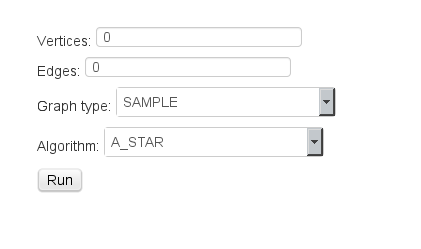
\includegraphics{img/input}
	\caption{Konfiguracja testowa do weryfikacji poprawnej instalacji aplikacji.}
	\label{fig:konfiguracja}
\end{figure}

Rysunek \ref{fig:wyniki} prezentuje wygląd strony z wynikami dla {\it Sample graph} oraz {\it A*}.

\begin{figure}[!h]
	\centering
	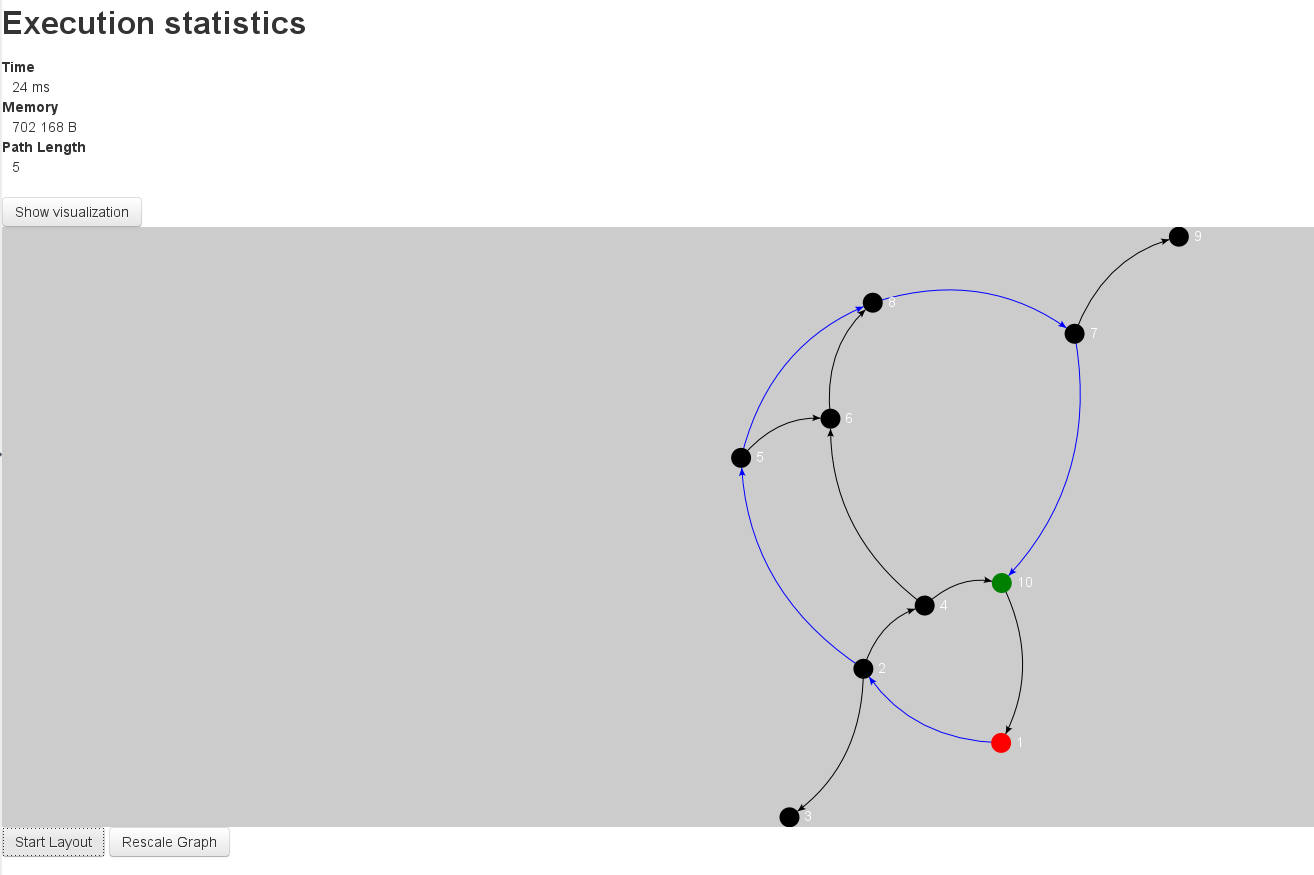
\includegraphics[width=\linewidth]{img/results}
	\caption{Przykładowy wynik planowania.}
	\label{fig:wyniki}
\end{figure}